\section{Composite}

% Description of the design pattern

\subsection*{Role}


\subsection*{Example}

\begin{figure}[htb]
    \centering
    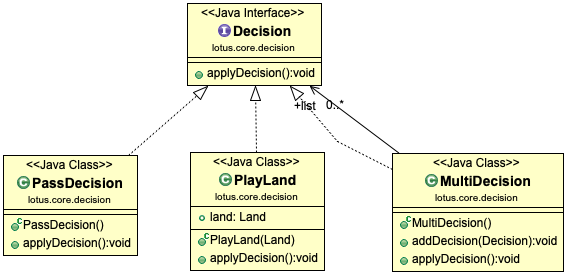
\includegraphics[width=0.8\columnwidth]{images/composite.png}
    \caption{Composite design pattern in the project \textit{lotus}}
    \label{fig:abstract_factory}
\end{figure}

%--------------------------------------------------------------------------------------------%

\begin{figure}[!tbp]
\centering
\lstset{language=Java, stepnumber=1, showspaces=false, showstringspaces=false,breaklines=true}
\begin{lstlisting}
public class MultiDecision implements Decision {
	public ArrayList<Decision> list = new ArrayList<Decision>();
	
	public void addDecision(Decision d) {
		list.add(d);
	}
 
	public void applyDecision() {
		for(Decision d : list) {
			d.applyDecision();
		}
	}
}
\end{lstlisting}
\caption{MultiDecision.java}
\label{}
\end{figure}

%--------------------------------------------------------------------------------------------%

\begin{figure}[!tbp]
\centering
\lstset{language=Java, stepnumber=1, showspaces=false, showstringspaces=false,breaklines=true}
\begin{lstlisting}

public class PlayLand implements Decision {
	public Land land;
	public PlayLand(Land l) {
		land = l;
	}
	public void applyDecision() {
		ChangeZone eff = new ChangeZone(land,land.zone,land.owner.inPlay);
		eff.resolve();
	}
}
\end{lstlisting}
\caption{PlayLand.java}
\label{}
\end{figure}

%--------------------------------------------------------------------------------------------%

\begin{figure}[!tbp]
\centering
\lstset{language=Java, stepnumber=1, showspaces=false, showstringspaces=false,breaklines=true}
\begin{lstlisting}

public class PassDecision implements Decision {
	public void applyDecision() {
		// Decision to pass, ie do nothing
	}
}

\end{lstlisting}
\caption{PassDecision.java}
\label{PassDecision.java}
\end{figure}

%--------------------------------------------------------------------------------------------%